\setchapterpreamble[u]{%
\dictum[Johann Wolfgang von Goethe]{Es ist nicht genug, zu wissen, man muß auch anwenden; es ist nicht genug, zu wollen, man muß auch tun. \dots}}
\chapter{Implementierung} \index{Implementierung}\label{kap:implementierung}

Dieses Kapitel beschreibt die Implementierung. 

\section{Configuration Management und Setup}\index{Configuration Managment}

\subsection{Maven}\index{Maven}
Maven ist ähnlich wie Ant ein Build und Deployment Werkzeug. Darüberhinaus ist es ein Dependency Management Werkzeug. Das bedeutet, dass Maven die abhängigen Artefakte und deren Versionen verwalten kann. 

\subsection{Apache Tomcat}\index{Apache Tomcat}
Als Web Container wird der \gls{Apache Tomcat} in der Version 7 eingesetzt. 

\subsection{Java 6}

\section{Web Service}\index{Web Service}\index{REST!RESTful Web Service}\label{kap:webservice}

Wie in Kapitel \todotext{XXX} erwähnt, wurde entschieden einen \gls{REST}ful Web Service zu erstellen. Dafür wurde das Jersey-Framework ausgewählt.

Folgende Schritte sind notwendig um einen \gls{REST}ful Webservice mit Jersey zu erstellen: 

\subsection{Servlet Konfiguration in web.xml} \index{Jersey}

In die Konfigurationsdatei web.xml des Webcontainers (hier \gls{Apache Tomcat}) muss das Servlet für \gls{Jersey} hinzugefügt werden, so dass \gls{Web Service} Anfragen an dieses Servlet möglich sind. 

\autoref{lst:jerseywebxmlconfig} zeigt den Ausschnitt aus der web.xml des \gls{PLIB}-Projektes. 

 \begin{lstlisting}[caption=Jersey Servlet Konfiguration in web.xml, language=XML, label=lst:jerseywebxmlconfig]
 <!-- configure jersey REST-Web Service Servlet -->
    <servlet>
        <servlet-name>jersey-servlet</servlet-name>
        <servlet-class>com.sun.jersey.spi.container.servlet.ServletContainer</servlet-class>
        <init-param>
            <param-name>com.sun.jersey.config.property.packages</param-name>
            <param-value>de.feu.plib.webservice.rest</param-value>
        </init-param>
        <load-on-startup>1</load-on-startup>
    </servlet>
 \end{lstlisting}   
 
Ferner muss in der web.xml ein sogenannter \enquote{Mappingeintrag} angelegt werden. Hierdurch wird dem Web Server mitgeteilt, bei zu welchem Servlet Anfragen an eine bestimmte URL zur Verarbeitung geleitet werden sollen. 
 
  \begin{lstlisting}[caption=Jersey Servlet Mappingkonfiguration in web.xml, language=XML, label=lst:jerseywebxmlconfigmapping]
    <servlet-mapping>
        <servlet-name>jersey-servlet</servlet-name>
        <url-pattern>/rest/*</url-pattern>
    </servlet-mapping>
 \end{lstlisting}  
 
Das Konfigurationbeispiel in \autoref{lst:jerseywebxmlconfigmapping}  besagt, dass das Servlet mit dem Namen \enquote{jersey-servlet}, welches im Beispiel \autoref{lst:jerseywebxmlconfig}  konfiguriert wurde, alle Anfragen mit der URL \enquote{/rest/*} entgegennehmen soll. Das Muster \enquote{/rest/*} bedeutet, das beliebige URLs nach /rest/ akzeptiert werden. Zum Beispiel: /rest/webservice oder /rest/service/name.

Unter der Annahme, dass die Applikation auf dem lokalem Rechner installiert wurde und auf Port 8080 lauscht, der Applikationskontext\footnote{XXX} \enquote{plib-characteristic-query} ist, ergibt sich als aktuelle Gesamt-URL für den Web Service der Applikation \enquote{http://localhost:8080/plib-characteristic-query/rest/}.
\index{Apache Tomcat!Applikationskontext} \todotext{Applikationskontext footnote}

\subsection{Web Service Klasse}
Der Einstiegspunkt für den \gls{Web Service} ist eine Klasse. Eine Applikation kann mehrere solcher Einstiegspunkte haben. Damit nun die Navigation von der URL der Anfrage zur entsprechenden Klasse funktioniert, wird jede Klasse mittels Annotation markiert und ein weiterer Pfad-Präfix definiert. Das Beispiel 
\autoref{lst:jerseywebservice} zeigt, dass mittels @Path der Suffix /ws definiert wird. 
  \begin{lstlisting}[caption=Jersey Web Service Klasse, language=Java, label=lst:jerseywebservice]
...
@Path("/ws")
public class QueryService {
...
 \end{lstlisting}  
 
Somit ergibt sich als aktuelle Gesamt-URL für den Web Service der Applikation \\  \enquote{http://localhost:8080/plib-characteristic-query/rest/ws}.
 
Der nächste Schritt ist nun, die entsprechenden Methode zu definieren, welche die Anfrage final entgegennimmt und verarbeitet (siehe \autoref{lst:jerseymethode}). 
 
  \begin{lstlisting}[caption=Jersey Methode, language=Java, label=lst:jerseymethode]
    @POST
    @Path("/query")
    @Consumes("application/xml")
    @Produces(MediaType.APPLICATION_XML)
    public String query(String queryXML) {
        LOGGER.info("Incoming query XML content :" + queryXML);
        QueryType queryType = unmarshall(queryXML);
        LOGGER.info("QueryType: " + queryType);
        CatalogueType catalogue = queryPipe.filter(queryType);

        LOGGER.info("Filled Catalogue: " + catalogue);
        String marshalledCatalogue = marshall(catalogue);

        LOGGER.info("Marshalled catalogue: " + marshalledCatalogue);
        return marshalledCatalogue;
    }
 \end{lstlisting}  

Die Konfiguration der Methode wird über \Gls{Annotation} vorgenommen. Nachfolgend die Erklärung der \Gls{Annotation} aus \autoref{lst:jerseymethode}.

\begin{description}
\item[@POST] Definiert die \gls{HTTP-Methode}. Hier POST. Einige weitere Möglichkeiten des HTTP-Protokolls sind GET, PUT und DELETE
\item[@Path('/query')] Definiert den URL-Pfad Suffix für diese Methode. Um diese Methode als Web Service via HTTP aufzurufen lautet die finale URL \enquote{http://localhost:8080/plib-characteristic-query/rest/query}. 
\item[@Consumes('application/xml')] Definiert den \gls{MIME-Type}\footnote{Internet Media Type oder auch Content-Type.}, welcher von diesem Service (diese Methode) konsumiert werden kann. Wird ein anderer Typ als POST an diesen Service geliefert, weist der Service diese Anfrage ab. 
\item[@Produces(MediaType.APPLICATION\_XML)] Definiert den \gls{MIME-Type} des Inhaltes, der vom Service als Antwort zurückgeliefert wird.  
\end{description}
\index{HTTP-Methode!GET}\index{HTTP-Methode!POST}\index{HTTP-Methode!PUT}\index{HTTP-Methode!DELETE}
\index{MIME-Type}

% 
\section{Query-Verarbeitung}

Der \gls{Web Service}, welcher in \autoref{kap:webservice} beschrieben ist, nimmt in der Applikation das Query-XML File entgegen. 
Die Struktur des XML-Files ist durch die query.xsd vorgegben \citep[27]{iso29002-31}. 

Der nächste Schritt ist es, diese XML zu Verarbeiten. Dazu muss das xml geparsed und die Informationen des Queries in ein entsprechendes Modell überführt werden. Diesen Prozess nennt man \gls{Unmarshalling}. 

Die folgenden Schritte müssen für das Unmarshalling durchgeführt werden.

\begin{enumerate}
\item Ein Modell in Java erstellen
\item XML parsen und in das Modell überführen
\item Validierung des Modells gemäß der Regeln in Schema-Datei
\end{enumerate}

%modell
\subsection{Modell-Generierung}

Ein entsprechend valides Model anhand der XSD manuell in Java aufzubauen wäre sehr mühsam und fehleranfällig. Java liefert mit der JAXB Bibliothek die Möglichkeit die Modellklassen von Java aus den XSDs zu generieren.

\subsubsection{Benötigte XSD-Dateien}

Die XSD-Dateien der ISO 29002-31 wurden freundlicherweise von Dr. Gerry Radack von der ECCMA zur Verfügung gestellt. 

Die query.xsd referenziert die weiteren folgenden Schema-Dateien:
\begin{itemize}
\item basic.xsd
\item identifier.xsd
\item catalogue.xsd
\item value.xsd
\end{itemize}

\subsubsection{Generierung mit JAXB}\index{Codegenerierung}

Die Generierung startet man als Java Kommando in der Konsole, siehe \autoref{lst:jaxbgeneratemodel}.

\begin{lstlisting}[caption=JAXB Modellgenerierung von der Konsole, language=sh, label=lst:jaxbgeneratemodel]
xjc query.xsd -d plib-characteristic-data/ 
\end{lstlisting}

\subsubsection{Problem Namensräume}
Bei der Generierung wurde die folgende Fehlermeldung angezeigt:

\enquote{[ERROR] The package name iso.std.iso.ts.\_29002.\_\_-31.ed\_1.tech.xml\_schema.query used for this schema is not a valid package name. line 18 of file query.xsd}
  
Der Grund für den Fehler ist, dass in der query.xsd die \glslink{Namespace}{Namensräume} wie in  \autoref{lst:queryschemanamespace} definiert sind. Da JAXB die \Glspl{Namespace} nutzt um die entsprechenden Paketstrukturen für die Modelle in Java zu erstellen, schafft es JAXB nicht, diese in entsprechende valide Form umzuwandeln. Man erkennt es daran, dass aus \enquote{urn:iso:std:iso:ts:29002:-31:ed-1:tech:xml-schema:query} in der Fehlermeldung \enquote{iso.std.iso.ts.\_29002.\_\_-31.ed\_1.tech.xml\_schema.query} wird\footnote{Java Paketnamen enthalten als Trenner zwischen den Ebenen einen Punkt. Valide wäre z.B. iso.std.iso.ts.query}. Der Bindestrich vor der 31 ist nicht als erstes Zeichen eines  Unterpaketnamens erlaubt. Wenngleich man hier erwarten würde, dass dies abgefangen und entsprechend der Umwandlungsregeln in valide Bezeichner konvertiert wird, so wäre dennoch eine Benamung der Pakete in der Form unübersichtlich.  \index{Namespace}

\code{public void doThat()}

\begin{lstlisting}[caption=query.xsd Namespace Definitionen, language=XML, label=lst:queryschemanamespace]
<xs:schema xmlns:xs="http://www.w3.org/2001/XMLSchema"
           xmlns:qy="urn:iso:std:iso:ts:29002:-31:ed-1:tech:xml-schema:query"
           xmlns:cat="urn:iso:std:iso:ts:29002:-10:ed-1:tech:xml-schema:catalogue"
           xmlns:val="urn:iso:std:iso:ts:29002:-10:ed-1:tech:xml-schema:value"
           xmlns:bas="urn:iso:std:iso:ts:29002:-4:ed-1:tech:xml-schema:basic"
           xmlns:id="urn:iso:std:iso:ts:29002:-5:ed-1:tech:xml-schema:identifier"
           targetNamespace="urn:iso:std:iso:ts:29002:-31:ed-1:tech:xml-schema:query" elementFormDefault="qualified">
    <xs:import namespace="urn:iso:std:iso:ts:29002:-4:ed-1:tech:xml-schema:basic" schemaLocation="basic.xsd"/>
    <xs:import namespace="urn:iso:std:iso:ts:29002:-5:ed-1:tech:xml-schema:identifier" schemaLocation="identifier.xsd"/>
    <xs:import namespace="urn:iso:std:iso:ts:29002:-10:ed-1:tech:xml-schema:catalogue" schemaLocation="catalogue.xsd"/>
    <xs:import namespace="urn:iso:std:iso:ts:29002:-10:ed-1:tech:xml-schema:value" schemaLocation="value.xsd"/>
    ...
</xs:schema>    
\end{lstlisting}

Für dieses Problem gibt es zwei Lösungsoptionen. Entweder die Namespace-Definitionen aller Namespaces in den XSD-Dateien anpassen oder die XSD-Dateien in der Form belassen und einen programmatischen Weg finden um die Namespaces umzudefinieren. 

Das Anpassen aller XSD-Dateien hat zwei große Nachteile.
\begin{enumerate}
\item Es ist aufwändig und fehleranfällig alle Dateien anzupassen. Diese haben wie in \autoref{lst:queryschemanamespace} zu sehen, Abhängigkeiten untereinander.
\item Änderungen an der lokalen Schemadatei machen mögliche spätere Integrationen einer neuen XSD-Version des ISO-Komitees schwierig.
\end{enumerate}

Besser wäre es, wenn die Generierung konfigurierbar ist. \gls{JAXB} ermöglicht mit einem sogenanntem Binding-File, die Namespaces abzuändern. \autoref{lst:bindingfile} zeigt die Konfiguration. Die Generierung kann mit dem Shell-Befehl \enquote{xjc -b binding.xjb -d gen-src query.xsd} gestartet werden. \index{Binding} \index{JAXB}

\begin{lstlisting}[caption=Binding File binding.xjc, language=XML, label=lst:bindingfile]
<?xml version="1.0" encoding="UTF-8"?>
<jaxb:bindings xmlns:jaxb="http://java.sun.com/xml/ns/jaxb"
               xmlns:xsd="http://www.w3.org/2001/XMLSchema"
               xmlns:xjc="http://java.sun.com/xml/ns/jaxb/xjc"
               jaxb:version="2.0">
  <jaxb:bindings schemaLocation="query.xsd" node="/xsd:schema">
    <jaxb:schemaBindings>
      <jaxb:package name="de.feu.plib.xml.query" />
    </jaxb:schemaBindings>
  </jaxb:bindings>
  <jaxb:bindings schemaLocation="basic.xsd" node="/xsd:schema">
    <jaxb:schemaBindings>
      <jaxb:package name="de.feu.plib.xml.basic" />
    </jaxb:schemaBindings>
  </jaxb:bindings>
  <jaxb:bindings schemaLocation="catalogue.xsd" node="/xsd:schema">
    <jaxb:schemaBindings>
      <jaxb:package name="de.feu.plib.xml.catalogue" />
    </jaxb:schemaBindings>
  </jaxb:bindings>
  <jaxb:bindings schemaLocation="identifier.xsd" node="/xsd:schema">
    <jaxb:schemaBindings>
      <jaxb:package name="de.feu.plib.xml.identifier" />
    </jaxb:schemaBindings>
  </jaxb:bindings>
  <jaxb:bindings schemaLocation="value.xsd" node="/xsd:schema">
    <jaxb:schemaBindings>
      <jaxb:package name="de.feu.plib.xml.value" />
    </jaxb:schemaBindings>
  </jaxb:bindings> 
  
      <jaxb:globalBindings>
         <!-- let the classes implement serialiseable -->
        <jaxb:serializable uid="1" />
          <!-- let the classes extend own abstract class for providing some extra functionality for each one -->
     </jaxb:globalBindings>  
</jaxb:bindings> 
\end{lstlisting}

Wie man erkennen kann, wird für jede Schema Datei ein eigener Paketname definiert. Das hat den Vorteil, dass die einzelnen Datentypen aus den jeweiligen XSD-Dateien passend in eigene Pakete generiert werden und nicht alle in ein Verzeichnis. Das ist deutlich übersichtlicher. 

Die Modell-Dateien werden folgendermaßen abelegt:

\begin{description}
\item[query.xsd] de.feu.plib.xml.query
\item[basic.xsd] de.feu.plib.xml.basic
\item[catalogue.xsd] de.feu.plib.xml.catalogue
\item[identifier.xsd] de.feu.plib.xml.identifier
\item[value.xsd] de.feu.plib.xml.value
\end{description}

Zeile 6-10 aus \autoref{lst:bindingfile} zeigt wie im Binding-File ein anderer Paketname für die Datei query.xsd definiert werden kann. 

\subsection{Einbinden in Buildprozess mit Maven}\index{Maven}\index{Buildprozess}
Da als Build-Werkzeug \gls{Maven} verwendet wird, kann der gesamte Generierungsprozess darüber abgebildet werden. 

\subsubsection{Separates Source-Verzeichnis}
Die Standardprojektform eines Maven-Projektes hat einen sogenannten Source-Folder (src). Darin befindet sich ein main-Folder. Dort werden die Klassen der Applikation abgelegt. Ferner beinhaltet der src-Folder einen test-Folder. Darin werden Testklassen abgelegt. 
Damit die generierten Sourcen klar getrennt sind von den anderen Source-Dateien, soll ein separates Source-Verzeichnis angelegt werden. Der weiterer Vorteil ist, dass dieser Folder beispielsweise auch vom Versionskontrollsystem ausgenommen werden kann, da diese Klassen während des Build-Prozesses jeweils generiert werden und somit keiner Versionierung bedürfen. Das wäre aufwändiger zu realisieren, wenn die Dateien exakt im gleichen Source-Folder generiert würden wo alle anderen Source-Dateien liegen\footnote{Hinweis: Moderne Versionskontrollsysteme wie das eingesetzte GIT ermöglicht es nach Mustern Dateien oder Ordner von der Versionierung auszunehmen. Allerdings müsste das hier auf Paketbasis erfolgen, sozusagen ab de.feu.plib.xml.*, das macht die Umgebung im Ganzen komplexer}. 

Maven bietet mittels des Plugins \enquote{build-helper-maven-plugin} die Möglichkeit, dies zu erzeugen. 
Die generierten Sourcen der XSD-Dateien werden in ein separates Verzeichnis namens \enquote{generated} erzeugt (siehe \autoref{lst:buildhelperplugin}). 

\begin{lstlisting}[caption=Build Helper Maven Plugin, language=, label=lst:buildhelperplugin]
<plugin>
    <groupId>org.codehaus.mojo</groupId>
    <artifactId>build-helper-maven-plugin</artifactId>
    <executions>
        <execution>
            <id>add-source</id>
            <phase>generate-sources</phase>
            <goals>
                <goal>add-source</goal>
            </goals>
            <configuration>
                <sources>
                    <source>src/main/generated</source>
                </sources>
            </configuration>
        </execution>
    </executions>
</plugin>
\end{lstlisting}

\subsubsection{JAXB Maven Plugin}

Um JAXB mit \gls{Maven} zu nutzen, muss das \gls{Maven}-Plugin \enquote{maven-jaxb2-plugin} in die \gls{pom} eingetragen werden. \autoref{lst:jaxbplugin} zeigt den XML-Auschnitt aus der \gls{pom}. \index{Maven!pom.xml}

\begin{lstlisting}[caption=JAXB Maven Plugin, language=XML, label=lst:jaxbplugin]
            <plugin>
                <groupId>org.jvnet.jaxb2.maven2</groupId>
                <artifactId>maven-jaxb2-plugin</artifactId>
                <version>0.8.0</version>
                <configuration>
                    <schemaDirectory>src/main/resources/schema</schemaDirectory>
                    <generateDirectory>src/main/generated</generateDirectory>
                    <removeOldOutput>true</removeOldOutput>
<!-- we do not use bindingDirectory as if we put the binding.xjb in the schema directory it will be taken -->
<!--                     <bindingDirectory>src/main/resources/binding</bindingDirectory> -->

<!--  Setting the generated package in pom will override what you set in binding.xjb file, thus commented out -->
<!--                     <generatePackage>de.feu.plib.jaxb</generatePackage> -->
                    <strict>false</strict>
                    <extension>true</extension>
                    <plugins>
                        <plugin>
                            <groupId>org.jvnet.jaxb2_commons</groupId>
                            <artifactId>jaxb2-basics</artifactId>
                            <version>0.6.2</version>
                        </plugin>
                        <plugin>
                            <groupId>org.jvnet.jaxb2_commons</groupId>
                            <artifactId>jaxb2-basics-annotate</artifactId>
                            <version>0.6.2</version>
                        </plugin>
                    </plugins>
                    <args>
                        <arg>-Xannotate</arg>
                        <arg>-XtoString</arg>
                    </args>
                </configuration>
                <executions>
                    <execution>
                        <id>generate</id>
                        <goals>
                            <goal>generate</goal>
                        </goals>
                    </execution>
                </executions>
            </plugin>    
\end{lstlisting}

\subsection{Abfrage der PLIB Prozeduren}

Die Anforderung ist es, so weit wie möglich die vorhandenen Prozeduren aus der Arbeit von Herrn Mende zu nutzen. 

Die Prozeduren von Herrn Mende nehmen einen sogenannten Externen Identifier entgegen. Dieser identifiziert eindeutig eine Instanz eines Teils. 
Beispiel: Ich habe das Konzept \enquote{Sechskantschraube} und in der Teiledatenbank gibt es davon genau eine gespeicherte Instanz, also eine Schraube mit definierten Werteeigenschaften. 

Zur Abfrage stehen folgende Oracle-Prozeduren zur Verfügung:

\begin{description}
\item[GET\_PROP\_VALS\_STRING] Nimmt als IN-Parameter eine Externe Produkt-ID entgegen und liefert eine Tabelle vom Typ PROP\_STRING\_NTT zurück. 
Diese Tabelle beinhaltet die folgenden Werte: 
  \begin{description}
  \item[IRDI] xxx
  \item[VALUE] xxx
  \item[UNIT] xxx
  \item[PREFIX] xxx
  \item[TOLERANCE] xxx
  \item[VALUE\_ID] xxx
  \end{description}

\todotext{Attribute beschreiben}  

\item[GET\_PROP\_VALS\_NUMBER]  xxx
\item[GET\_PROP\_VALS\_REFERENCES]  xxx
\item[GET\_PROP\_VALS\_LIST\_NUMBER] xxx
\item[GET\_PROP\_VALS\_LIST\_STRING] xxx
\item[GET\_PROP\_VALS\_MULTILIST\_NUMBER] xxx
\item[GET\_PROP\_VALS\_MULTILIST\_STRING]  xxx
\item[GET\_PROP\_VALS] xxx  
\end{description}

\todotext{Attribute beschreiben} 

\subsubsection{Problem - Externer Identifier}

Hier stellt sich das Problem, dass eine query.xsd generell immer auf die IRDI eines Konzeptes basiert. 
Beispiel: \enquote{Gib mir bitte alle Instanzen und Werte der Eigenschaften des Klassenkonzeptes mit dem Identifier 0173-1\#01-BAD803\#2 (Skalpell)}
Der Query des Standards fragt folglich explizit nach den Instanzen eines Konzeptes (hier Skalpell). Die Prozeduren benötigen allerdings einen nicht im Standard definierten Identifier einer konkreten Instanz, um alle Eigenschaftswerte zu ermitteln. 

\subsubsection{Lösung}

Zwei Lösungsoptionen stellen sich hier zur Auswahl:
\begin{enumerate}
\item Anpassen der Datenbank-Prozeduren, so dass anstatt eines externen Identifiers eine IRDI entgegengenommen werden kann.
\item Separate Abfrage an die Datenbank in der Applikation realisieren. Diese Abfrage ermittelt anhand der vom Query übergebenen IRDI alle externen Identifier der Instanzen dieses Konzeptes. Anschließend können die Prozeduren aufgerufen werden.   
\end{enumerate}

Es wurde die Lösung Nummer zwei gewählt. Hierfür gibt es mehrere Gründe. Der Hauptgrund ist, dass zum Zeitpunkt der Erstellung dieser Arbeit, die Abschlussarbeit von Herrn Mende noch nicht abgeschlossen ist. Es ist damit nicht auszuschließen, dass sich Prozeduren oder Logik in den Prozeduren zu einem späteren Zeitpunkt noch ändern. Das ist im Prinzip kein Problem, da diese Arbeit sich auf einen bestimmten Entwicklungsstand der Arbeit von Herrn Mende bezieht, allerdings wird in der Zukunft versucht, die neuere Version von Herrn Mende in diese Arbeit zu integrieren, wird es sehr schwierig und aufwändig dies zu bewältigen, wenn im Rahmen dieser Arbeit die Prozeduren geändert werden. Man stände vor dem Problem, dass beide Seiten die Basis modifiziert haben. 
Ein weiterer Grund für die separate Abfrage ist, dass dies in der Ebene der Applikationslogik für einen Nicht-Oracle Experten einfacher zu implementieren, und damit weniger fehleranfällig ist. Die Prozeduren sind bereits sehr komplex und im Detail nicht einfach zu verstehen. 
Ferner stellt diese Abfrage eine Teilfunktionalität dar und ist somit prima separat testbar.  

Das \autoref{lst:getexternalids} zeigt den SQL-Query der Lösung des Problems.

\begin{lstlisting}[caption=JAXB Maven Plugin, language=SQL, label=lst:getexternalids]
SELECT o.DI_ID FROM DE_CLASS c, DO_OBJECT o WHERE c.ID = o.C_ID AND c.IRDI = ?
\end{lstlisting}

Zur Erklärung des \autoref{lst:getexternalids}:
DI\_ID ist der Attributsname des oben genannten externen Identifiers einer Instanz. Das Prädikat IRDI = ? nimmt die IRDI des eigentlichen Queries gemäß query.xsd entgegen. Das Ergebnis ist eine Liste der externen Identifier, welche dann je an die Prozedur übergeben werden können. 

Um zu verstehen, wie diese Abfrage in der Applikation im Kontext verwendet wird, sei auf das Sequenzdiagramm in \autoref{fig:sequenzdiagrammsimplequery} verwiesen. 

\begin{figure}[htbp]
	\centering
		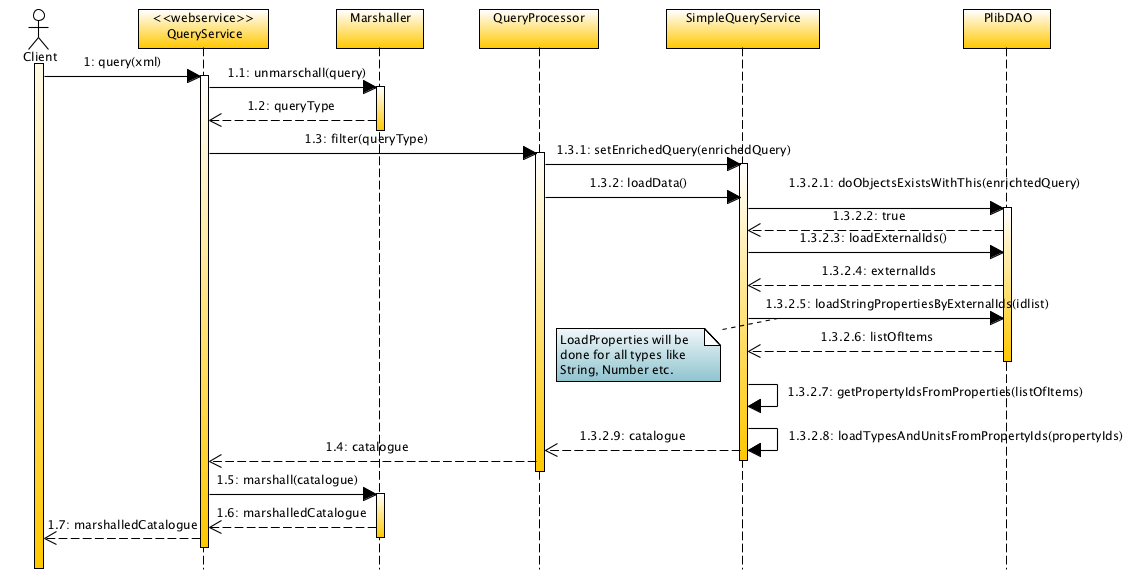
\includegraphics[width=0.99\textwidth]{images/plib_simple_query_sequence_diagram.png}
		\caption{Sequenzdiagramm Simple Query}
	\label{fig:sequenzdiagrammsimplequery}
\end{figure}

\section{Zusammenfassung des Kapitels}



